\documentclass[11pt, a4paper, twoside, openright]{article} %draft

\usepackage{graphicx,color}
\usepackage{listings}
\usepackage{hyperref}
\usepackage{subfig}

\usepackage{color}
\definecolor{lightgray}{rgb}{.9,.9,.9}
\definecolor{darkgray}{rgb}{.4,.4,.4}
\definecolor{purple}{rgb}{0.65, 0.12, 0.82}

\lstdefinelanguage{JavaScript}{
  keywords={typeof, new, true, false, catch, function, return, null, catch, switch, var, if, in, while, do, else, case, break},
  keywordstyle=\color{blue}\bfseries,
  ndkeywords={class, export, boolean, throw, implements, import, this},
  ndkeywordstyle=\color{darkgray}\bfseries,
  identifierstyle=\color{black},
  sensitive=false,
  comment=[l]{//},
  morecomment=[s]{/*}{*/},
  commentstyle=\color{purple}\ttfamily,
  stringstyle=\color{blue}\ttfamily,
  morestring=[b]',
  morestring=[b]"
}

\lstset{
   language=JavaScript,
   backgroundcolor=\color{lightgray},
   extendedchars=true,
   basicstyle=\footnotesize\ttfamily,
   showstringspaces=false,
   showspaces=false,
   numbers=left,
   numberstyle=\footnotesize,
   numbersep=9pt,
   tabsize=2,
   breaklines=true,
   showtabs=false,
   captionpos=b
}
\usepackage{amssymb, amsmath, array}



\begin{document}

% Example of title page for the projects carried out within DEDIS
% Copied from lasec 

% Simply include it in your mastex tex file: 
%        % Example of title page for the projects carried out within DEDIS
% Copied from lasec 

% Simply include it in your mastex tex file: 
%        % Example of title page for the projects carried out within DEDIS
% Copied from lasec 

% Simply include it in your mastex tex file: 
%        \input{cover}


% Updated October 2016


\newcommand{\logoepfl}[0]{
  \begin{center}
    
\includegraphics[width=4cm]{logo_epfl_coul.eps}
  \end{center}
  \vspace{0.3cm}
  \hrule
}
\newcommand{\project}[1]{
  \begin{center}
    \large{#1}
  \end{center}
  \vspace{1cm}
}
\newcommand{\department}[1]{
  \begin{center}
    \large{#1}
  \end{center}
}
\newcommand{\lab}[1]{
  \begin{center}
    \large{#1}
  \end{center}
}
\newcommand{\supervisor}[3]{
  \begin{center}
    \begin{normalsize}{
        \bf #1}\\#2\\#3
    \end{normalsize}
  \end{center}
}
\renewcommand{\author}[1]{
  \begin{center}
    \Large{#1}
  \end{center}
  \vspace{0.5cm}
}
\renewcommand{\title}[1]{
  \vspace{3cm}
  \begin{center}
    \huge{#1}
  \end{center}
  \vspace{1.7cm}
}
\renewcommand{\date}[2]{
  \begin{center}
    \normalsize{#1 #2}
  \end{center}
  \vspace{0.5cm}
}


\thispagestyle{empty}


% begin title page
  \logoepfl
  
  \title{Explore cross-platform mobile platforms}
  
  \author{Louis-Maxence Garret}
  \department{School of Computer and Communication Sciences}
  \lab{Decentralized and Distributed Systems lab}
  \project{Master Optional Project}
  
  \date{January}{2019}

  \begin{center}
    \begin{tabular}{cc}
      \begin{tabular}{p{4.0cm}}
        \supervisor{Responsible}{Prof. Bryan Ford}{EPFL / DEDIS}
      \end{tabular}&
      \begin{tabular}{p{4.0cm}}
        \supervisor{Supervisor}{Linus Gasser}{EPFL / DEDIS}
      \end{tabular}
    \end{tabular}
  \end{center}

% end title page




% Updated October 2016


\newcommand{\logoepfl}[0]{
  \begin{center}
    
\includegraphics[width=4cm]{logo_epfl_coul.eps}
  \end{center}
  \vspace{0.3cm}
  \hrule
}
\newcommand{\project}[1]{
  \begin{center}
    \large{#1}
  \end{center}
  \vspace{1cm}
}
\newcommand{\department}[1]{
  \begin{center}
    \large{#1}
  \end{center}
}
\newcommand{\lab}[1]{
  \begin{center}
    \large{#1}
  \end{center}
}
\newcommand{\supervisor}[3]{
  \begin{center}
    \begin{normalsize}{
        \bf #1}\\#2\\#3
    \end{normalsize}
  \end{center}
}
\renewcommand{\author}[1]{
  \begin{center}
    \Large{#1}
  \end{center}
  \vspace{0.5cm}
}
\renewcommand{\title}[1]{
  \vspace{3cm}
  \begin{center}
    \huge{#1}
  \end{center}
  \vspace{1.7cm}
}
\renewcommand{\date}[2]{
  \begin{center}
    \normalsize{#1 #2}
  \end{center}
  \vspace{0.5cm}
}


\thispagestyle{empty}


% begin title page
  \logoepfl
  
  \title{Explore cross-platform mobile platforms}
  
  \author{Louis-Maxence Garret}
  \department{School of Computer and Communication Sciences}
  \lab{Decentralized and Distributed Systems lab}
  \project{Master Optional Project}
  
  \date{January}{2019}

  \begin{center}
    \begin{tabular}{cc}
      \begin{tabular}{p{4.0cm}}
        \supervisor{Responsible}{Prof. Bryan Ford}{EPFL / DEDIS}
      \end{tabular}&
      \begin{tabular}{p{4.0cm}}
        \supervisor{Supervisor}{Linus Gasser}{EPFL / DEDIS}
      \end{tabular}
    \end{tabular}
  \end{center}

% end title page




% Updated October 2016


\newcommand{\logoepfl}[0]{
  \begin{center}
    
\includegraphics[width=4cm]{logo_epfl_coul.eps}
  \end{center}
  \vspace{0.3cm}
  \hrule
}
\newcommand{\project}[1]{
  \begin{center}
    \large{#1}
  \end{center}
  \vspace{1cm}
}
\newcommand{\department}[1]{
  \begin{center}
    \large{#1}
  \end{center}
}
\newcommand{\lab}[1]{
  \begin{center}
    \large{#1}
  \end{center}
}
\newcommand{\supervisor}[3]{
  \begin{center}
    \begin{normalsize}{
        \bf #1}\\#2\\#3
    \end{normalsize}
  \end{center}
}
\renewcommand{\author}[1]{
  \begin{center}
    \Large{#1}
  \end{center}
  \vspace{0.5cm}
}
\renewcommand{\title}[1]{
  \vspace{3cm}
  \begin{center}
    \huge{#1}
  \end{center}
  \vspace{1.7cm}
}
\renewcommand{\date}[2]{
  \begin{center}
    \normalsize{#1 #2}
  \end{center}
  \vspace{0.5cm}
}


\thispagestyle{empty}


% begin title page
  \logoepfl
  
  \title{Explore cross-platform mobile platforms}
  
  \author{Louis-Maxence Garret}
  \department{School of Computer and Communication Sciences}
  \lab{Decentralized and Distributed Systems lab}
  \project{Master Optional Project}
  
  \date{January}{2019}

  \begin{center}
    \begin{tabular}{cc}
      \begin{tabular}{p{4.0cm}}
        \supervisor{Responsible}{Prof. Bryan Ford}{EPFL / DEDIS}
      \end{tabular}&
      \begin{tabular}{p{4.0cm}}
        \supervisor{Supervisor}{Linus Gasser}{EPFL / DEDIS}
      \end{tabular}
    \end{tabular}
  \end{center}

% end title page



\newpage
\thispagestyle{empty}
\tableofcontents{\protect\thispagestyle{empty}
\newpage
        
% Start page count
\setcounter{page}{1}

\section{Introduction}

%%% Motivation

Upon buying a second-hand car, in most cases, consumers wonder whether that particular car has been stolen in the past or holds some hidden flaws. Frauds are very common when it comes to previously owned vehicles and some examples include tampering with the readings of odometers, hiding maintenance details as well as the history of accidents.\\
\newline
This problem in the automotive industry costs the consumers, car dealers, manufacturers, insurance and leasing companies approximately between 5.6 and 9.6 billion euros per year in Europe \cite{Costs}.
Thus, the question that persists is how to fight these criminal deceptions and establish trust among the above-mentioned entities.\\
\newline
Our motivation is to create a solution that allows buyers to be confident in their purchase and owners to increase the value of their car. We propose a proof of concept that includes a blockchain for keeping maintenance data of cars in form of a digital registry, where the records persist forever and are resistant to manipulation.\\
\newline
The idea is to add maintenance reports for every regular vehicle inspection, as well as for every unexpected malfunctioning or car crash. Some of the data used in these reports is generated by IoT devices that measure mileage, score of well driving and other parameters when placed on a vehicle.\\ 
\newline
This documentation is structured to offer a background information about the blockchain technology in section~\ref{Background} and then introduce an overview of the project in section~\ref{Overview}.\\
\newline
Furthermore, in section~\ref{Implementation}, we cover the implementation details of our work, including the management of access rights, creation of digital contracts for enforcing specific performance, handling the private data and also the interaction between the users and the blockchain.\\
\newline
Finally, in section~\ref{Evaluation} we test and evaluate the behaviour of our system in larger networks and with parallel transactions. We utilize visualized charts in order to draw better conclusions and then we finish our work with future possibilities for improvement.\\
\newline
In summary, this project shows how the blockchain technology can be applied in other spheres of the real world (particularly in the automotive industry), and not only in the well known financial area, with the purpose of solving trust and fraud issues.
\newline
\section{SkipChain Explorer}
\newline
\subsection{Cothority Framework}
The Cothority project (collective authority) is a decentralized cryptography Framework developed by the Decentralized and Distributed Systems lab (DEDIS) at EPFL. The Framework \cite{cothority} will be used in the context of this project. In particular, the code in this repository allows the user to access the services of a cothority and/or run its own conode.
\newline
\subsection{Choosing the right components}
Before jumping into what Cothority has to offer, it is important to have an idea in mind of what we are working towards. This project uses \href{https://vuejs.org/}{Vue.js} and \href{https://vuetifyjs.com/en/}{Vuetify} for the application rendering. First of all, several existing Blockchain Explorer tools have been analyzed and reviewed, such as \href{https://etherscan.io/}{etherscan.io} and \href{https://blockexplorer.com/}{blockexplorer.com}, to help choosing the best features to be implemented.


The first draft contains the home page, where the latest blocks from the given SkipChain would be displayed with some of the most interesting and general information about each of these blocks.

In order to recreate this draft, it was necessary to do some initial research on which Vuetify components to use and then on how to interact with SkipChains.
\subsection{Talking to a SkipChain}
As a first step, everything needs to run locally to make sure it works as expected. A local Roster is set up (i.e a group of Cothority servers) with three running nodes:
\\
\begin{lstlisting}[language=bash]
  $ ./run_conode.sh local 3 3
\end{lstlisting}
Once the local Roster is all set, it is possible to start generating SkipChains via the SkipChain Manager (scmgr) tool.
Using the SkipChain Manager, the user can set up, modify and query SkipChains. The scmgr will be running on the local machine and it will communicate with one or more remote conodes. For it to work, the user needs the public.toml of a running cothority where he has the right to create a SkipChain or add new blocks.
This command allows the user to generate interesting SkipChains (in this example, a SkipChain with base 3 and height 4 is created):
\begin{lstlisting}[language=bash]
  $ scmgr s c -b 3 -he 4 
  ~/go/src/github.com/dedis/cothority/conode/public.toml
\end{lstlisting}
Once the SkipChain is created, scmgr will print out its ID, and the user can start adding data into the chain:
\begin{lstlisting}
  $ scmgr s b add --data 'Hello' { skipchain id }
  $ scmgr s b add --data 'World' { skipchain id }
\end{lstlisting}
\subsection{Changing the Roster}
As mentioned previously, the Roster is the group of Cothority servers which will sustain the SkipChains. A button on the upper right of the page allows the user to change the Roster he wishes to connect to via a simple text field. In this project, the default Roster is set to be the following:
\begin{lstlisting}[language=JavaScript]
`
[[servers]]
  Address = "tls://gasser.blue:7002"
  Public = "036bf316e1ea6e7e99e0bb713419d16
            c0b6794bf9dc442cc4cf36c3f935e93cf"
  Description = "EPFL Cothority-server"
`
\end{lstlisting}
which allows the user to have access to the DEDIS' SkipChains.
\clearpage
\newpage
\subsection{Fetching the Blocks}
In this step, the https://www.overleaf.com/project/5c238c1dddbc4b53474c059cgoal is to interact with a SkipChain. However, as the web front-end is written in JavaScript using Vue.js and the back-end is written in Go, Protocol Buffers are needed.
Protocol Buffer messages are a fast way to allow back-end/front-end communication \cite{protobuf}.
To access a SkipChain's blocks the method \verb|GetUpdateChain| is used. A first surprise was to see that it didn't seem to load all of the chain's blocks. After some research, it was realized that this method returns all the blocks from the highest layer of forward links. In other words, all the blocks from the fastest SkipChain's traversal. 

Another option would have been to call \verb|GetSingleBlockByIndex|.
\\
Although this method returns all the blocks, it is based on an iterative call, and would therefore kill the essence of the SkipChain: a logarithmic chain traversal. Only the "main blocks" from these highest links were then kept.
In the home page, (\href{http://status.dedis.ch/ng/}{status.dedis.ch/ng}) the user is given the possibility to choose the SkipChain that he wishes to connect to. After selection, the latest blocks are displayed from the selected SkipChain, which are the blocks from the response of \verb|GetUpdateChain|.
\newline
\begin{figure}[h]
    \centering
    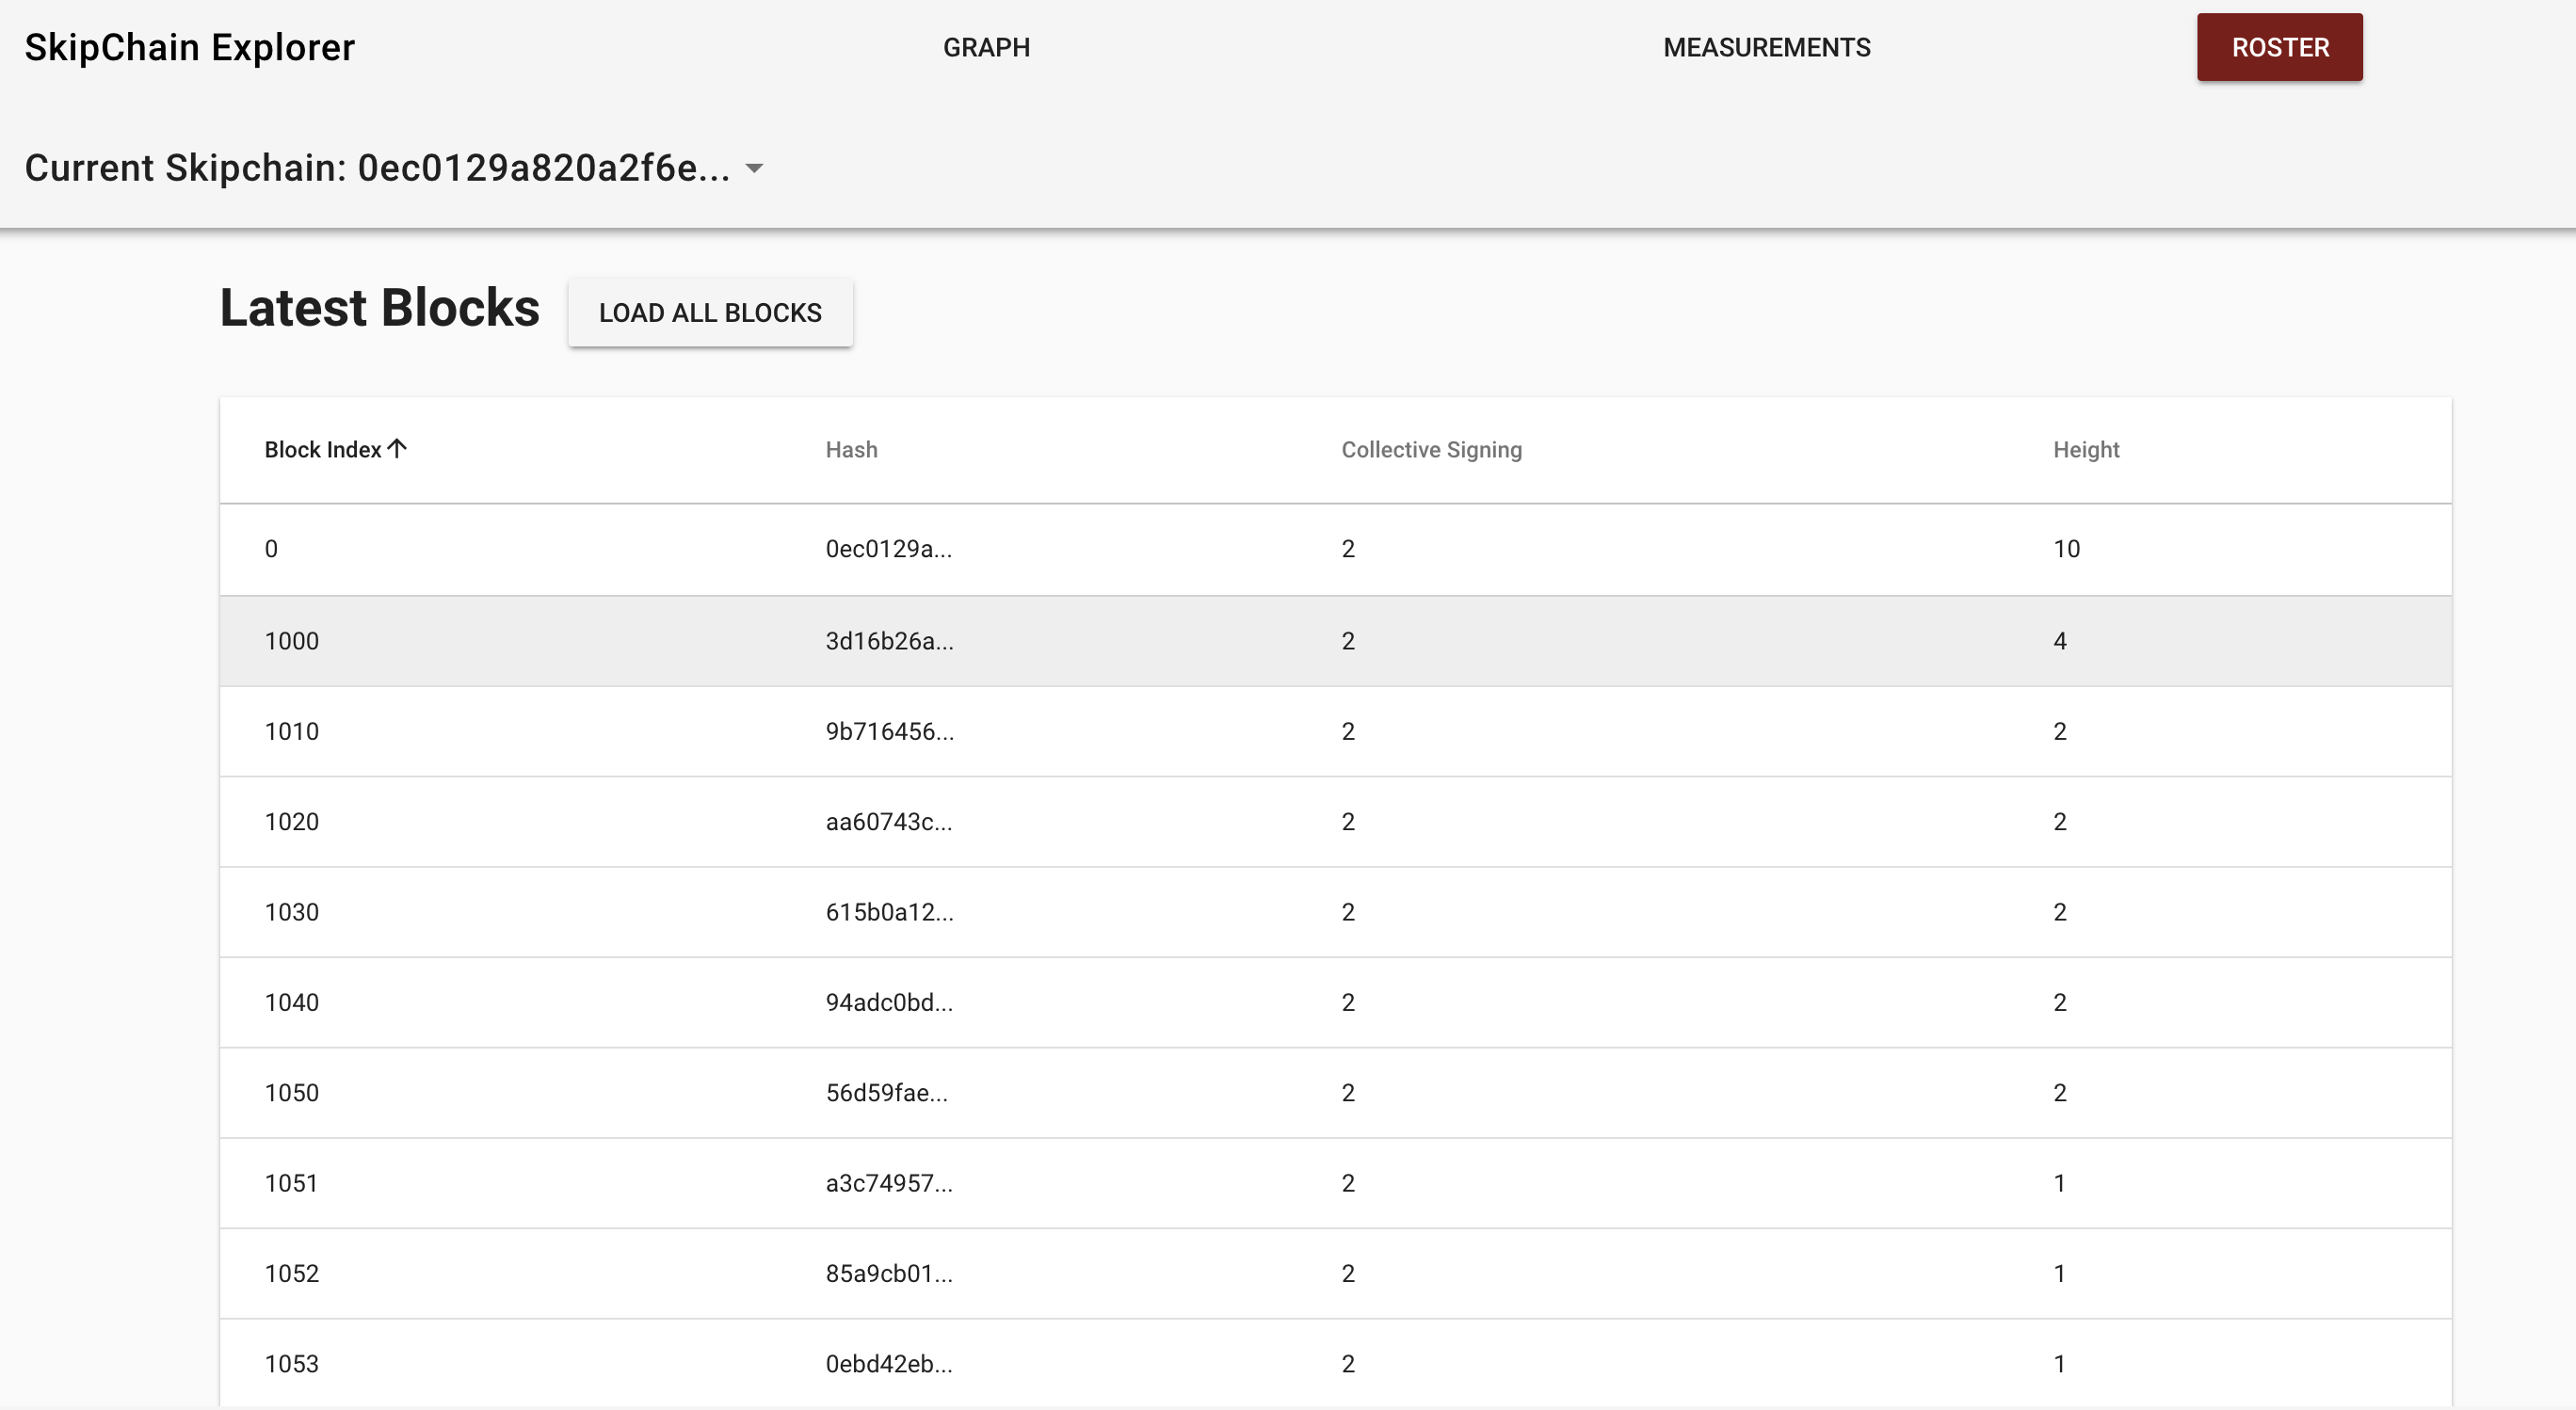
\includegraphics[width=\textwidth]{LatestBlocks}
    \caption{Homepage after SkipChain selection. Blocks and their main info are displayed}
    \label{fig:my_label}
\end{figure}
\clearpage
\subsection{Block Information}
The "Block Information" page is different for each block. It displays all the information considered interesting about the selected SkipBlock.

First of all, a method called \verb|getBlockByHash| has been created, which, given a hash, returns the corresponding SkipBlock. This method will be particularly useful when working with Backward and Forward links.


Once the user has selected the desired SkipChain, he can navigate through its blocks, which is where it becomes interesting. What information is contained in a given block? How many blocks are reachable via the Forward/Backward links?
The Block Information page gives the user the following:

\begin{figure}[h]
    \centering
    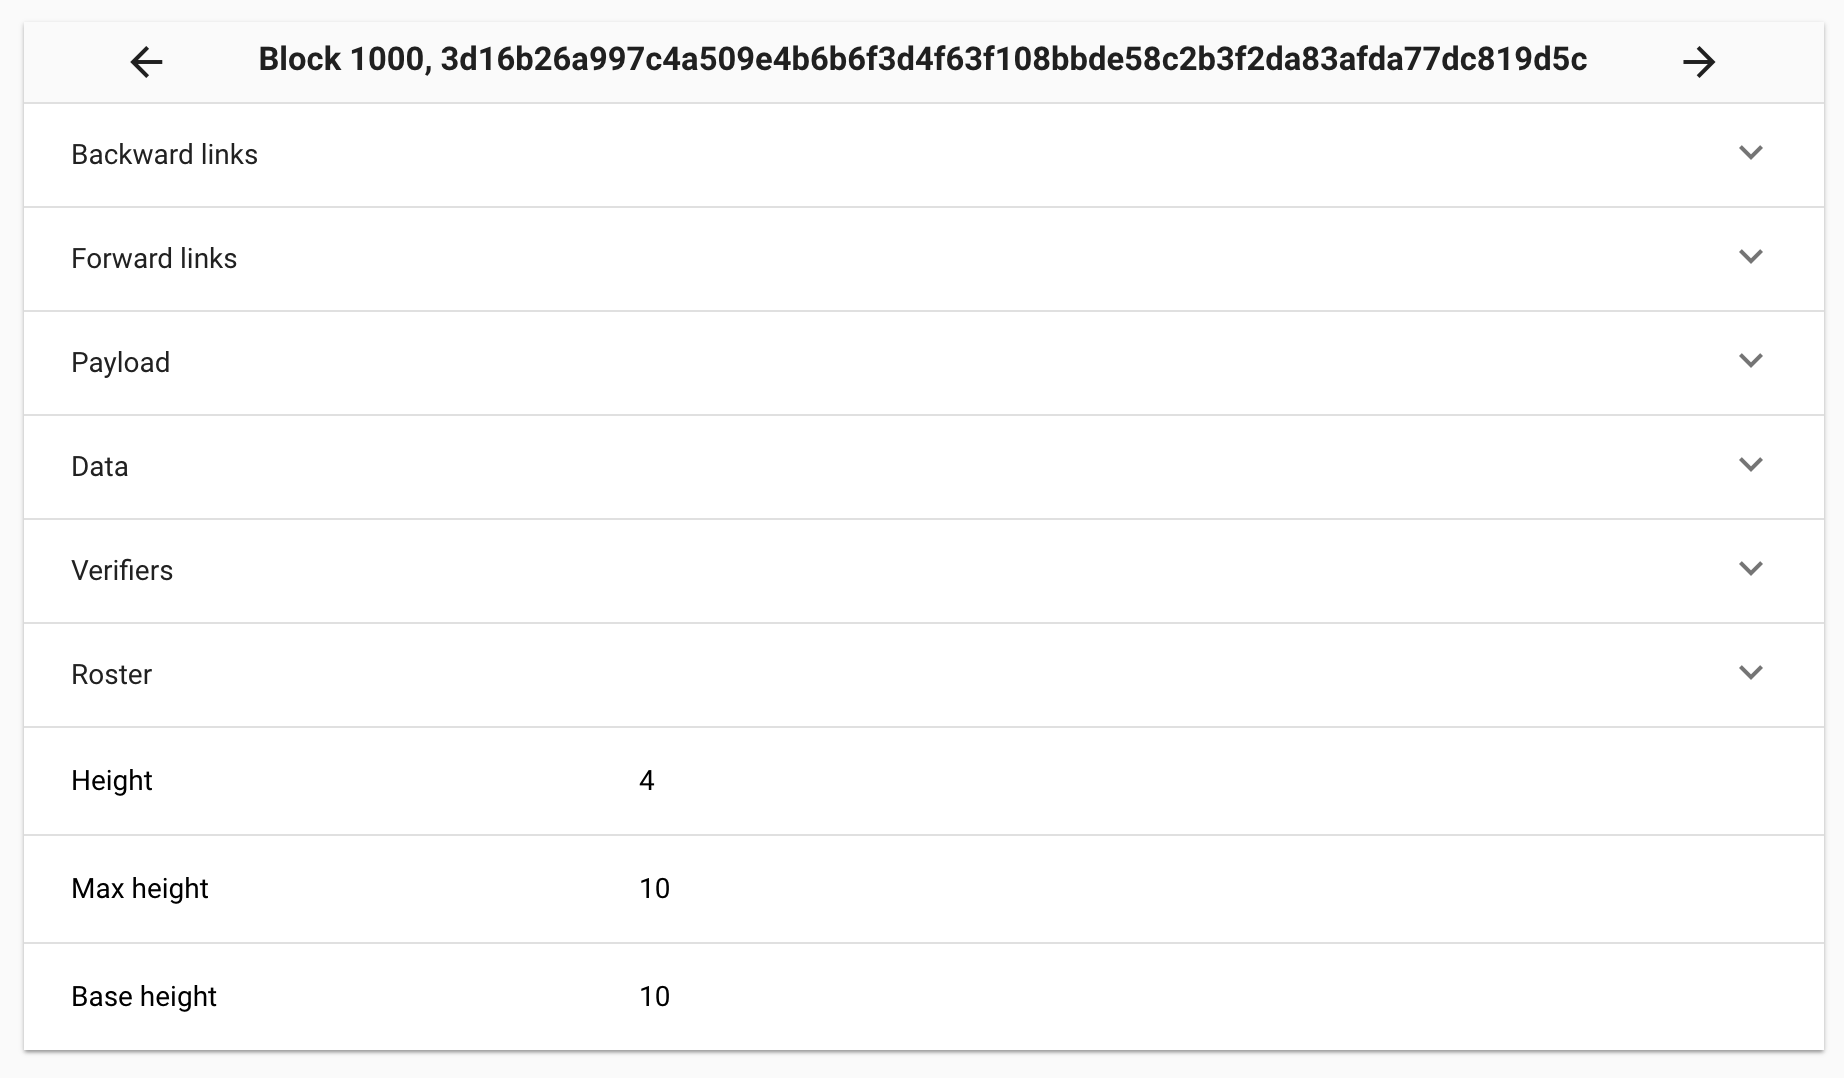
\includegraphics[width=\textwidth]{BlockInfo.png}
    \caption{Information page for a selected block}
    \label{fig:my_label}
\end{figure}
\newpage
\subsubsection{Backward and Forward links}


The Backward and Forward links of a block are displayed in function of their level. The higher the level the faster the SkipChain will be traversed, as it implies a bigger hop. The user can click on the link and he will be redirected to the correspondent block page. As Forward and Backward links are represented as hashes (and not SkipBlocks) of the block they point to, \verb|getBlockByHash| had to be used.
\begin{figure}[h]
    \centering
    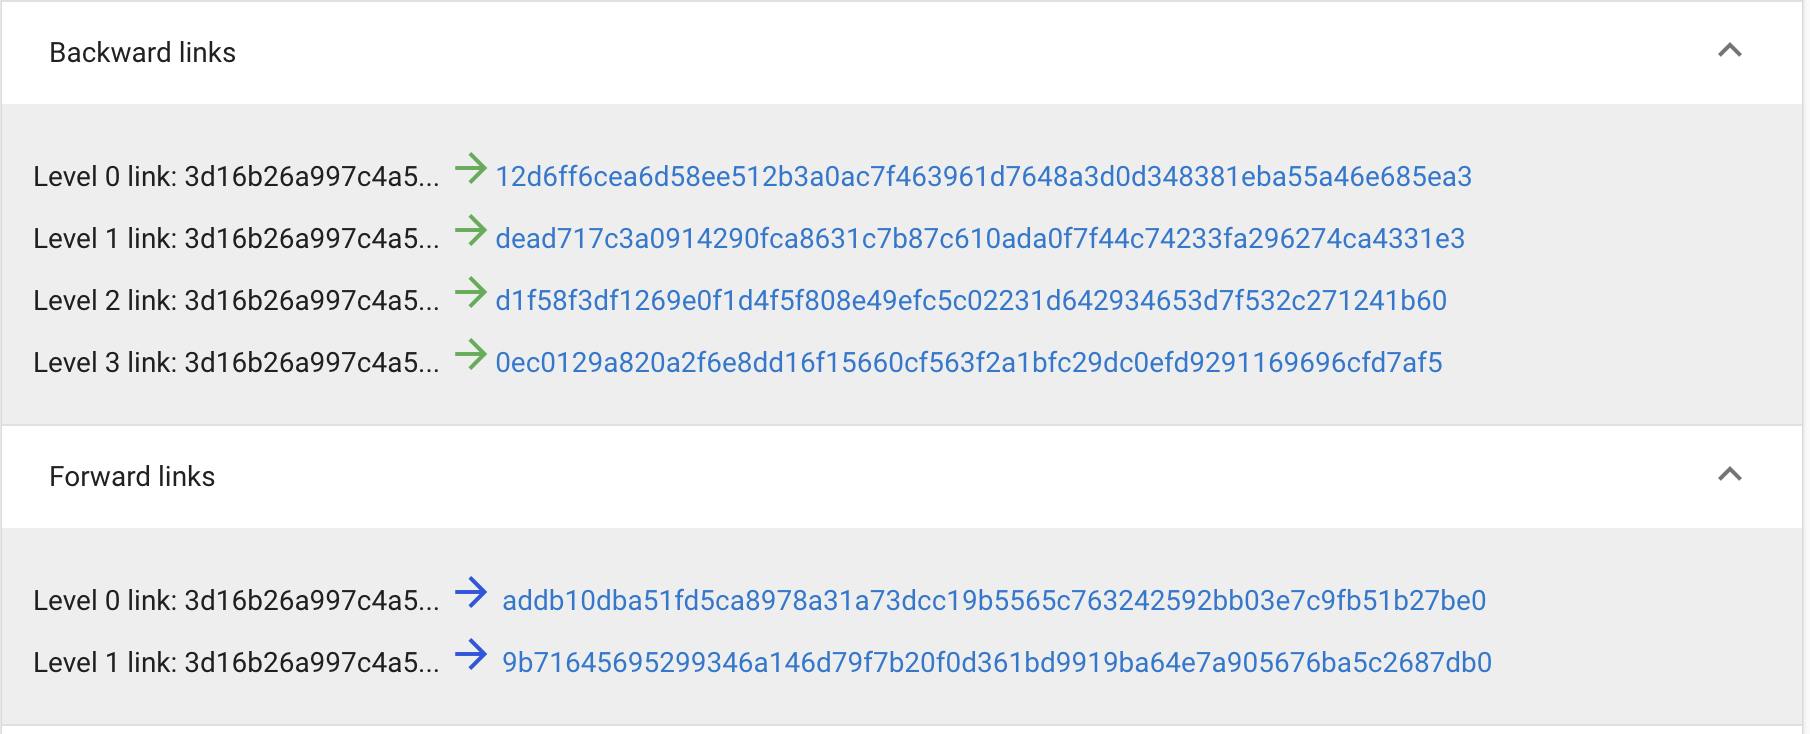
\includegraphics[width=\textwidth]{Links.png}
    \caption{Forward and Backward Links of a given block}
\end{figure}
\subsubsection{Payload and Data}

The Payload and Data correspond to the Data Body and Data Header of a SkipBlock. 
In the context of this project, there were two types of SkipChains: ByzCoin and non-ByzCoin chains.
A ByzCoin, by definition \cite{Byzcoin} is a Bitcoin-like crypto-currency enhanced with strong consistency, based on the principles of the well-studied Practical Byzantine Fault Tolerance (PBFT) \cite{BFT} algorithm. 
First of all, in the case of non-Byzcoin SkipBlocks the Payload field of the block is null and the Data field is left as a hex dump. 
\begin{figure}[h]
    \centering
    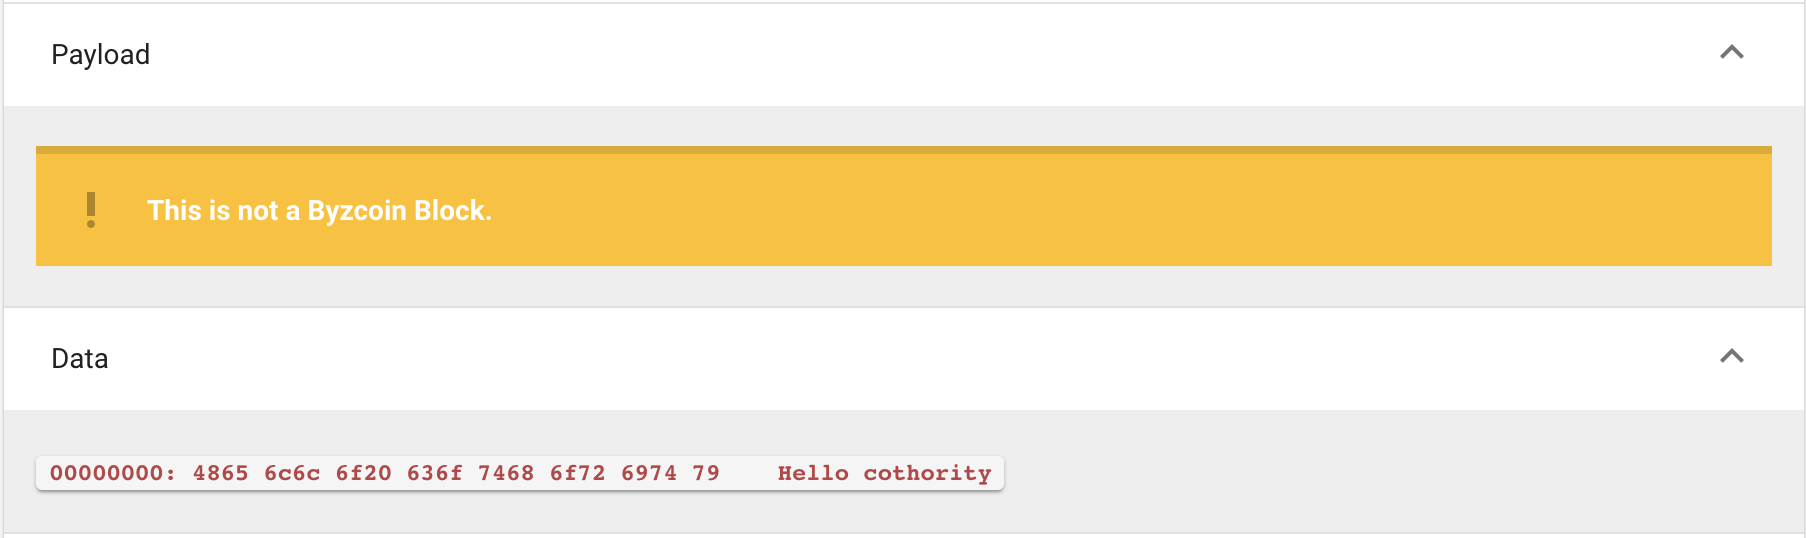
\includegraphics[width=\textwidth]{nonByzcoin.png}
    \caption{Data Body (Payload) and Header (Data) of a non-ByzCoin SkipBlock}
\end{figure}
\newpage
ByzCoin SkipBlocks are particularly interesting as they can hold multiple transactions per block.
As a second step of the project, once everything was working,  ByzCoin blocks have been decoded by recognizing whether there is a ByzCoin Verifier among the SkipChain's Verifiers set.
In order to work with ByzCoin, it was necessary to stay on the byzgen\_1810 branch, as it was stable. Decoding the Payload and Data of the SkipBlock becomes now more interesting.
\newline
\newline
\textbf{ByzCoin Data}
\newline
\newline
The following command allows us to inspect a block's Data (Data Header):
\begin{lstlisting}
    const headerLookup = protobuf.root.lookup('DataHeader')
    const header = headerLookup.decode(this.block.data)
\end{lstlisting}


The Data Header field for ByzCoin blocks contains four elements: three hashes: client transaction hash, state change hash and the trieroot defined as the following:
\begin{itemize}
    \item client transaction hash: a hash of all the client transactions listed in the Data Body (Payload) part of the SkipBlock
    \item state change hash: hash of the state change, which is either Create, Update or Remove
    \item Trieroot: hash of the Merkle trie root of Global State (whose value is determined by StateChange)
\end{itemize}
and one timestamp.\\
These values were left as they are, except for the timestamp which has been converted into readable format.
\begin{figure}[h]
    \centering
    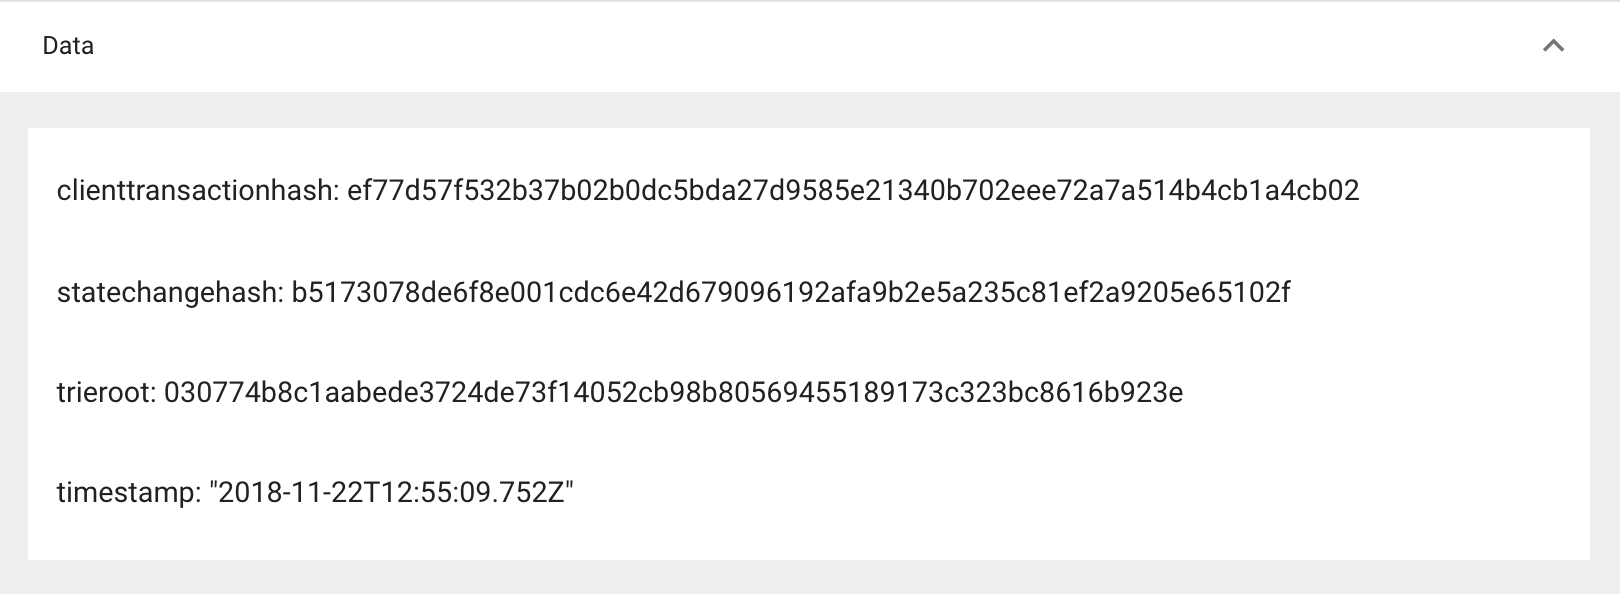
\includegraphics[width=\textwidth]{Header.png}
    \caption{Data Header of a ByzCoin SkipBlock}
\end{figure} 
\newline
\newline
\newline
\newline
\textbf{ByzCoin Payload}
\newline
\newline
As for the Data Body (Payload), we can inspect it with a similar command:
\begin{lstlisting}
    const bodyLookup = protobuf.root.lookup('DataBody')
    const body = bodyLookup.decode(this.block.payload)
\end{lstlisting}


The payload is displayed as a list of transactions, which can either be accepted or rejected. We have two types of transactions: Spawn and Invoke (we haven't worked with Delete transactions, as there were none available). Spawn and Invoke transactions both contain a list of instructions and a signature. The signature for each transaction is represented as a tuple of a Signature (UUID) and a Signer.
Spawn instructions are characterized by a contract id and an instance id (Figure~\ref{fig:Figure6}). Invoke instructions are characterized by a command (Figure~\ref{fig:Figure7}). All instructions then contain their arguments with name and value, which has been left under hexadecimal format.

\begin{figure}[h]
    \centering
    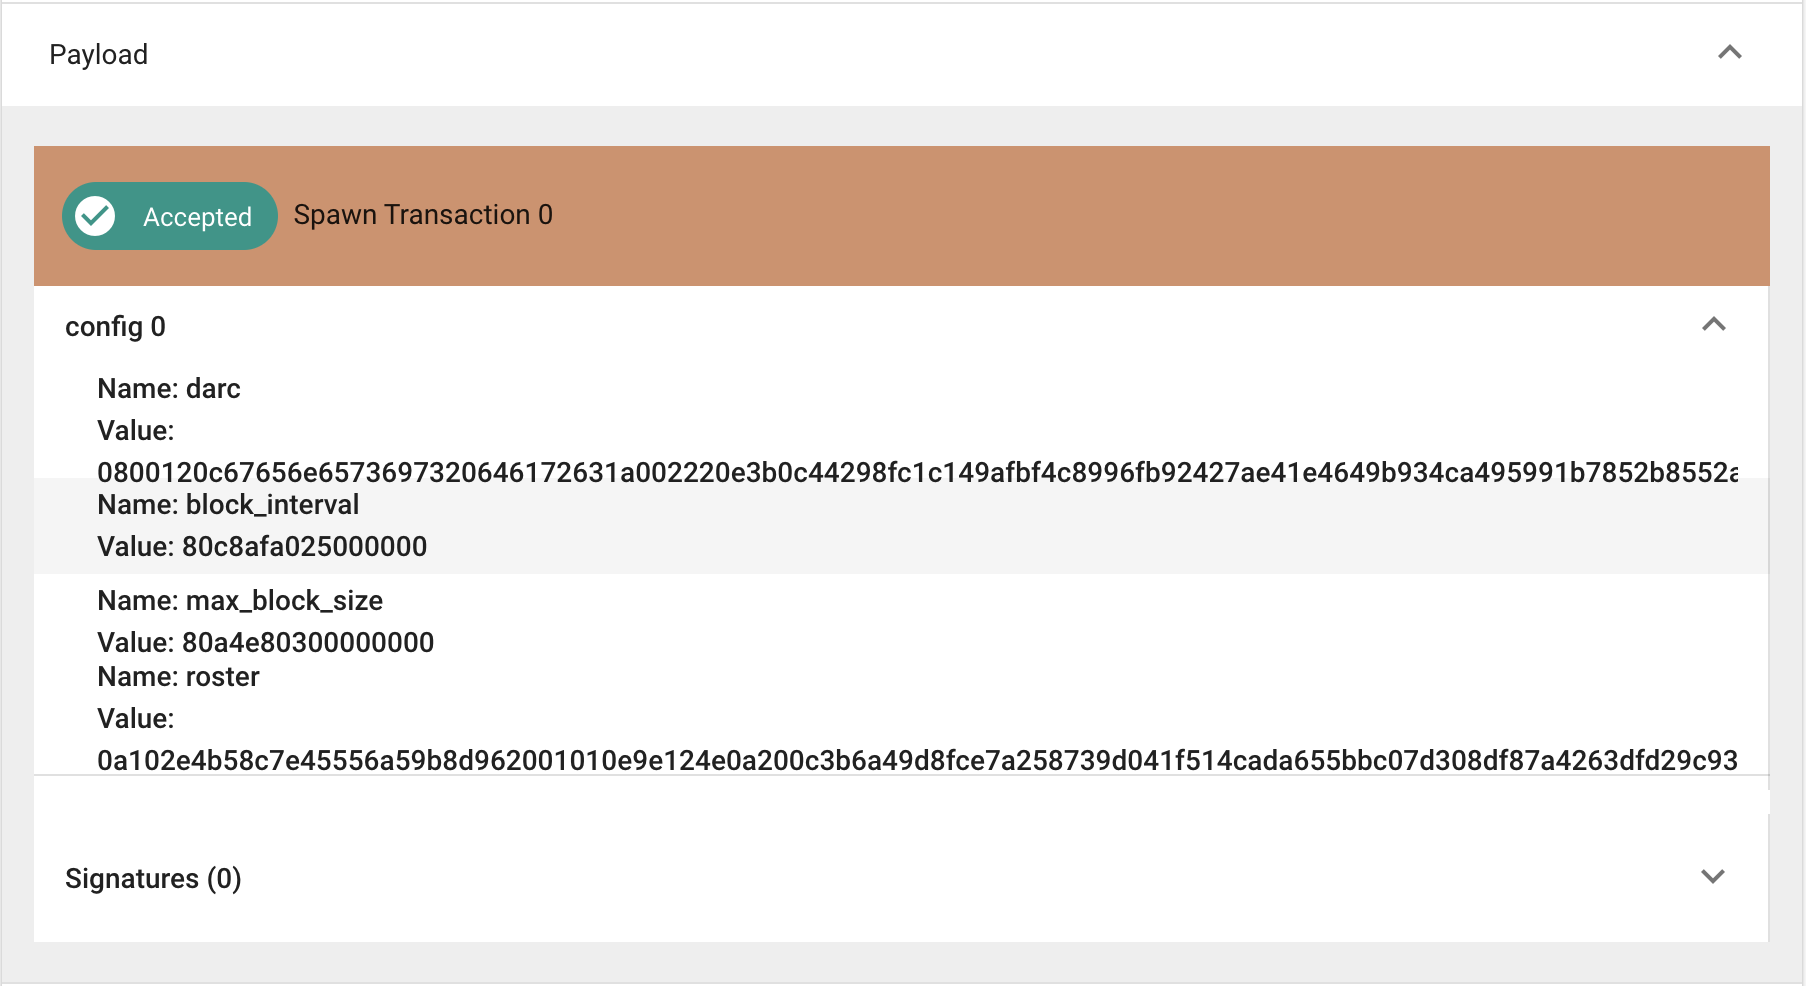
\includegraphics[width=\textwidth]{spanw.png}
    \caption{Payload of a ByzCoin SkipBlock as a Spawn Transaction with contract id "config" and instance id "0"}
    \label{fig:Figure6}
\end{figure}
\begin{figure}[h]
    \centering
    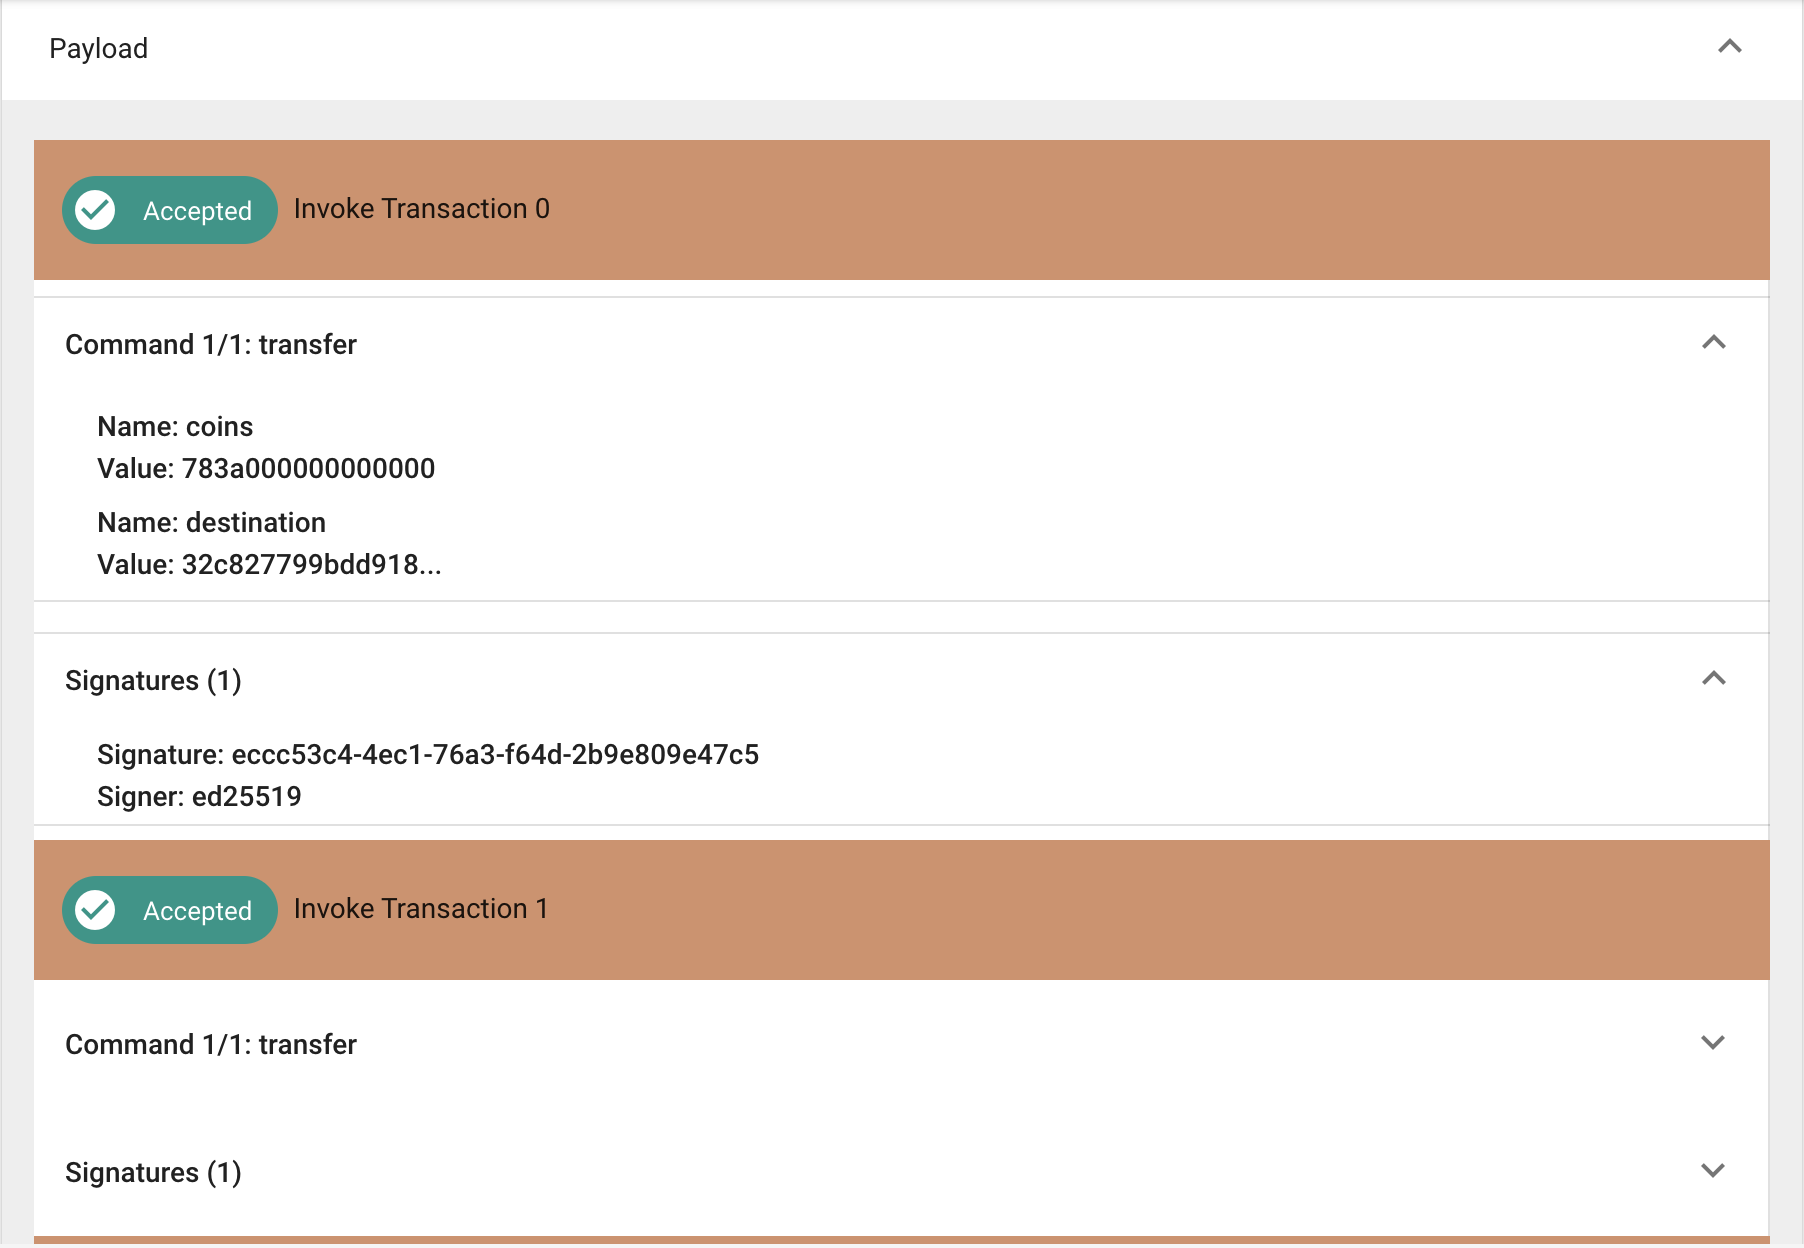
\includegraphics[width=\textwidth]{Transactions.png}
    \caption{Payload of a ByzCoin SkipBlock as list of Invoke transactions with "transfer" commands}
    \label{fig:Figure7}
\end{figure}
\newpage
\subsubsection{Verifiers}
Verifiers tell the user whether this is a ByzCoin block or not. So far, the block information page displays two kinds of Verifiers: Base Verifier and ByzCoin Verifier. Each Verifier is displayed as a UUID.

\begin{figure}[h]
    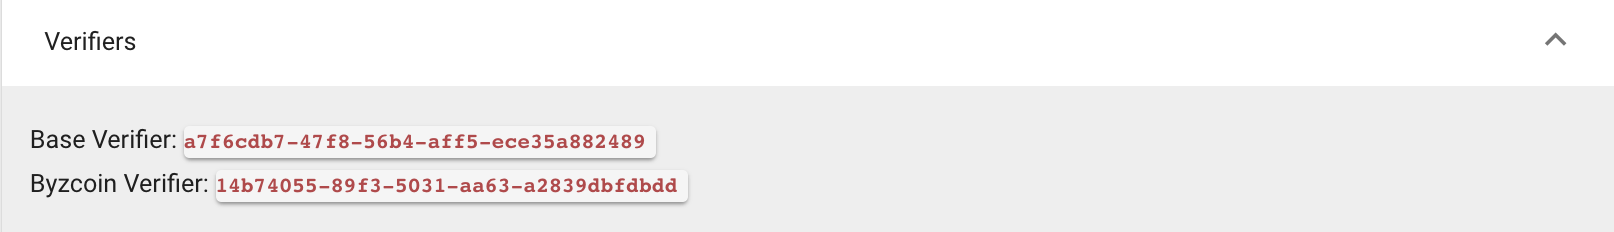
\includegraphics[width=\textwidth]{Verifiers.png}
    \caption{List of Verifiers for a ByzCoin SkipBlock}
\end{figure}
\subsubsection{The Roster}

In this part, we display the information relative to the Roster. A Roster is defined by its id and a set of conodes. Each conode has an id, an address, and a potential description. Each id is displayed as a UUID.
\begin{figure}[h]
    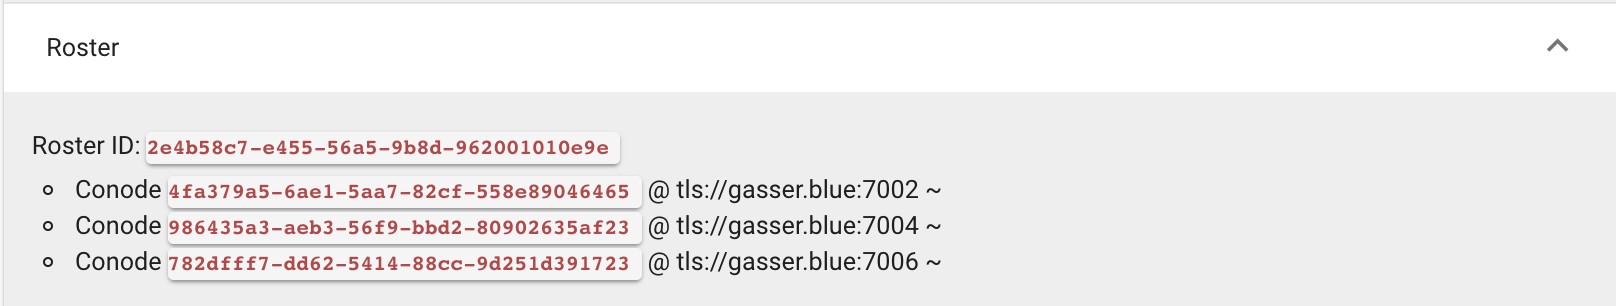
\includegraphics[width=\textwidth]{Roster.png}
    \caption{The Roster of a given block}
\end{figure}
\newpage
\subsubsection{Additional informations}

Additional information such as height, max height and base height give details about the current SkipChain and SkipBlock.
The bigger the base height, the longer the links between the blocks get. The bigger the maximum height, the longer the longest link gets and the more links a SkipBlock can have.
\begin{figure}[h]
    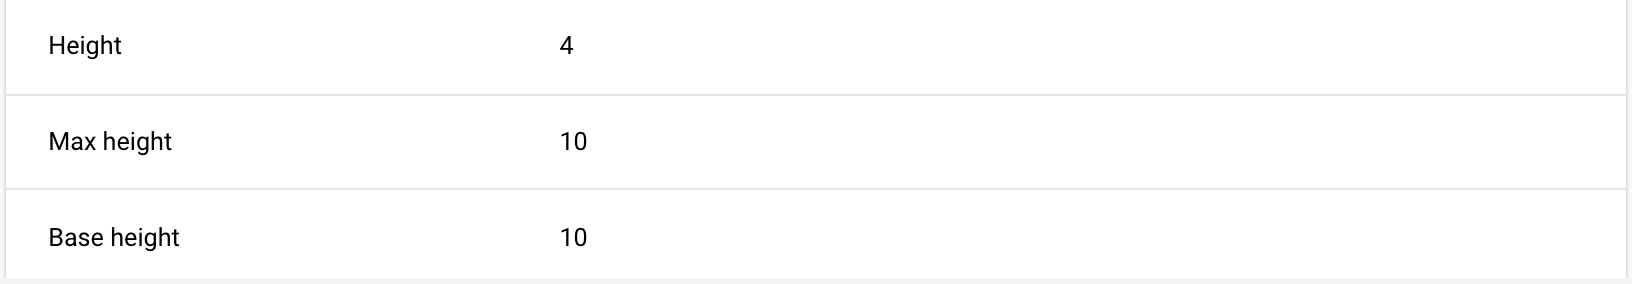
\includegraphics[width=\textwidth]{Additional.png}
    \caption{Other informations about the given block}
\end{figure}
\subsection{Unit Testing}
Part of this project was to implement unit tests in order to verify that everything is displaying accordingly.

Although Vue.js suggests its users to use Karma, this project uses Mocha for unit testing as it is more straightforward and the most used library.
Mocha has proven to be useful to cover the basic tests that were needed in this project. Two SkipBlocks that are connected to each other were saved in a `blocks.js` file. Overall, it has been certified that the Block Information page displays every item correctly, for instance the block's hash, the UUIDs of the Roster and Verifiers. It was also checked that the hashes of the Forward and Backward links were displayed as expected in the Block Information page.

A test coverage has also been implemented. Once the tests passed correctly, Travis was added into the project. Travis is a great way to check whether all tests pass without forcing the user to run them himself.
If the user wishes to test the code before pushing its changes, the following commands can be used:
\begin{lstlisting}[language=bash]
    $ yarn pretest --fix
    $ yarn test
    $ yarn coverage
    \end{lstlisting}
    
At the end, creating tests was a great learning. Knowing that everything works as expected and leaving the code in a good state for the next programmer is rewarding and necessary.
\subsection{Issues}
One idea was, in the Forward/Backward links part of the block information page, to show next to each link to which block index it redirects to. This way, it would allow the user to know that with a click he can go from block 0 to block 1000, for instance. However, as Forward/Backward links are represented as hashes and not SkipBlocks, it would be necessary to fetch the SkipBlock (using \verb|getBlockByHash|) to have access to its index, which would be time consuming. As a result, the index of the SkipBlocks are not displayed.

In this part, the reactivity of the components has major importance. The user must be able to navigate quickly between the blocks and the page design must be intuitive. Some bugs have been resolved, they resulted from a keying problem. Indeed, in Vue.js the pages update themselves based on a key given as input. If the programmer doesn't choose the right one it will result in a static page. 
\section{SkipChain Graph}
The goal of this part is to create a visual identity to each SkipChain, allowing the user to see its format and interact with it. 
First of all, we looked for different libraries that could help reaching this goal. At the end, it has been decided to use \href{https://d3js.org/}{D3}, a JavaScript library that helps bringing data to life. Although there is a lot to take from D3, it was important to stick to the basics and work from there. A method called \verb|getBlockByIndex| will be helpful in this part.
\subsection{Blocks and Links Representation}
To create the blocks and links, many instances have been used such as rectangle, line, polyline and polygon. The design has been inspired on the original paper \cite{paper}. For more usability, the graph has been changed from horizontally to vertically. This way, the user can scroll through the blocks more easily.
As a first step, all the blocks that had been fetched were displayed, that is the blocks that have been returned by the \verb|getUpdateChain| call. Indeed, as we remember, \verb|getUpdateChain| only returns the blocks from the highest Forward link traversal (see Figure~\ref{fig:main} (a)). In the graph, each block' size is represented as a multiple of its height and the blocks are ordered in function of their index. 

Once that was in place, the rest of the blocks (the un-fetched ones, non returned by the \verb|getUpdateChain| call) were displayed. The user has the possibility to fetch any of these blocks by clicking on it. These unloaded blocks are represented as grey squares. Unloaded blocks from higher layers (i.e they have forward links of level 1 or higher) are represented in light-pink. When the user clicks on a square, it fetches the corresponding block via a \verb|getBlockByIndex| call. The user can also have access to the information of a certain block by double-clicking it: he will be redirected to the information page of the  block in question.
We only display links from blocks that have been fetched.

\subsection{Usability}
A user might want to have an easy access to the latest block. As the graph visualization starts with the Genesis block, a button that allows the user to go directly to the bottom of the page was added. This way, one can directly access the end of the SkipChain (i.e the latest SkipBlock). The opposite has also been implemented, once at the bottom of the page, the user can go back to the top with a simple click.

One might also want to load the whole SkipChain, i.e all the grey squares, or at least its majority. For this purpose, two buttons were added:
\begin{itemize}
    \item Load Higher Traversal Blocks (see Figure~\ref{fig:main} (b))
    \begin{itemize}
        \item This button will fetch all the blocks from the non-zero link layers (represented in light-pink). That is, the only resulting unfetched blocks are the ones from the lowest layer.
        \item This feature allows the user to have a good visualization of the SkipChain without having to load it entirely.
    \end{itemize}
    \item Load All Blocks (see Figure~\ref{fig:main} (c))
    \begin{itemize}
        \item This button will fetch every single block form the corresponding SkipChain.
        \item A pop-up will appear to confirm the action. Indeed, if the Roster isn't potent enough, the web-browser might crash.
    \end{itemize}
\end{itemize}


\begin{figure}[htp]
\centering
\subfloat[]{\label{a}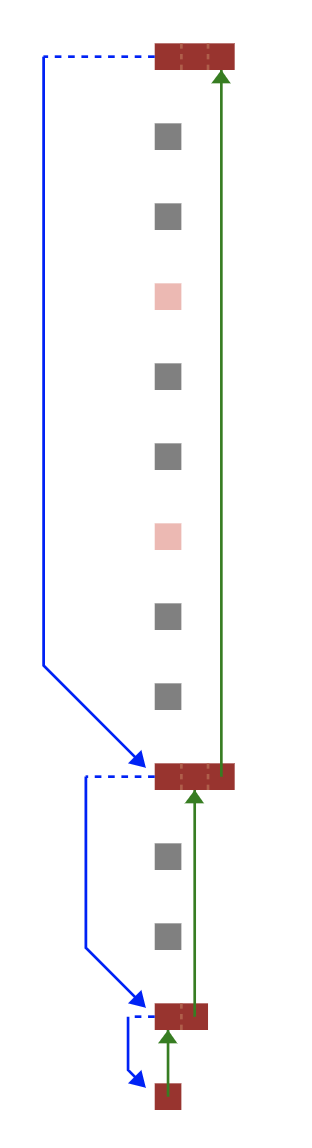
\includegraphics[width=.3\textwidth, height=400]{update.png}}\hfill
\subfloat[]{\label{main:b}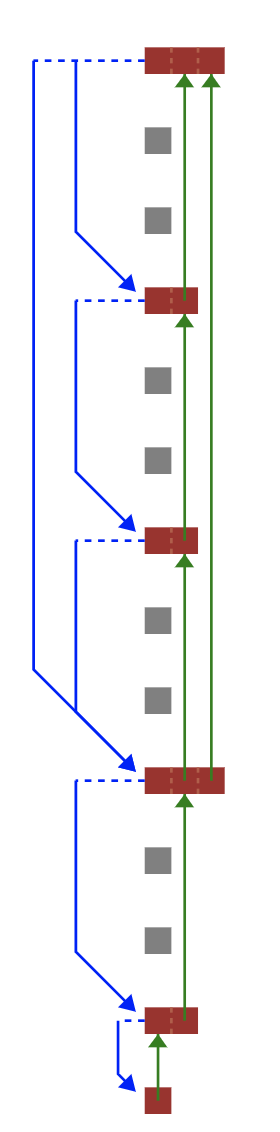
\includegraphics[width=.3\textwidth, height=400]{fetchmost.png}}\hfill
\subfloat[]{\label{main:c}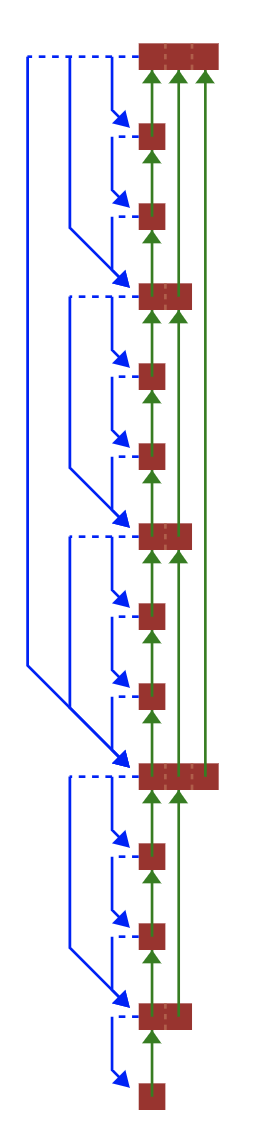
\includegraphics[width=.3\textwidth, height=400]{fetchall.png}}

\caption{The current SkipChain's graph after (a) loading the Graph page (b) fetching most SkipBlocks from highest link layers (c) fetching the whole Chain.}
\label{fig:main}

\end{figure}
\newpage
\subsection{Issues}
One issue has come up when creating all blocks. Indeed, once \verb|getUpdateChain| returned some blocks, it was necessary to artificially create the rest of the blocks (the unloaded ones) of the SkipChain in order to be able to display them as well on the graph. Meaning that there is an array called allBlocks containing either blocks (that have been fetched) either simple objects with the following definition:
\begin{lstlisting}
    { loaded: false, index: i, height: 1 }
\end{lstlisting}
The height is preset to 1 so they can be displayed as squares, but once the SkipBlock is fetched its real height is assigned to it.
At this moment, an indexing issue has been discovered: instead of showing a block's index i, it showed 2*i. After some research and re-reading of the code, to conclusion that has been made was that the problem came from the Protocol Buffering on the lab' side. Once this issue was taken care of, indexes were displayed as expected.

Some work has been done so that the SkipChain's Graph displays correctly on mobile platforms, by adapting its dimensions.

\newpage
\section{Measurements}
\subsection{Incentive}
So far, a visualization tool has been created for the SkipChains from a given Roster and their content. The SkipChain technology promises a faster chain traversal in logarithmic time in comparison to other BlockChain technologies.
Has this development been able to keep that feature? Are SkipChains still profitable and time-saving? To verify these hypothesis, a series of measurements has been conducted. The following is being computed:
\begin{itemize}
\item First of all, how much time does it take to traverse every Forward link layer. That is, how much time it takes to go from the Genesis block to the latest block on the given layer of Forward link. This is computed based on the \verb|getBlockByHash| method.
\item Then, it is interesting to see how long it takes to fetch every single block from the chain index by index, using \verb|getBlockByIndex|.
\item Finally, we measure how much time it takes to traverse the whole chain, how long it takes to get to the latest block starting at the Genesis block. To do so, we stay on the highest Forward link layer at all times. The search is done using \verb|GetBlockByHash|.
\end{itemize}
\subsection{Results}
We will observe the results in the largest SkipChain we have so far, which has 1'058 blocks to this date, and four different layers of Forward Links. It is relevant to note that this SkipChain has base 10 and height 10.
\\\\
\begin{figure}[h]
    \centering
    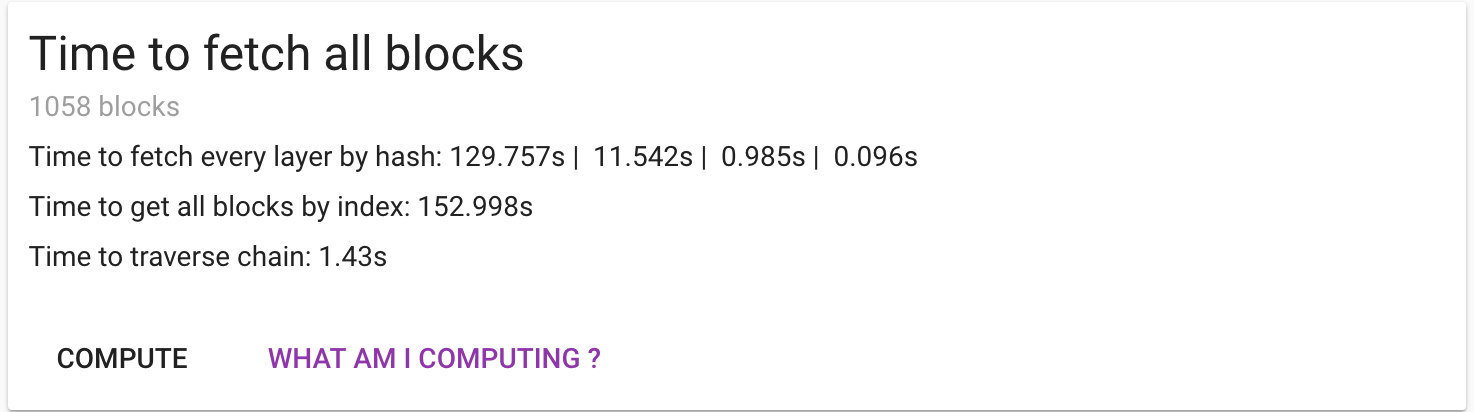
\includegraphics[width=\textwidth]{Measurements1058.png}
    \caption{Measurements for a 1'058 SkipBlocks SkipChain}
    \label{fig:Figure12}
\end{figure}

As we can see it takes up to 2 minutes (129.757 s) to traverse the lowest layer and 0.096 seconds to traverse the highest one with the \verb|getBlockByHash| call. It also takes up to 2 minutes (152.998 s) to fetch all blocks using \verb|getBlockByIndex|.
Finally, it takes a total of 1.43 seconds to traverse the whole chain.
It can indeed be concluded that using higher level Forward Links brings efficiency to the chain's traversal. More precisely, using the highest Forward links rather than sticking to the lowest level Forward link is more than ninety times more efficient ($\frac{129.757}{1.43} = 90.73$). Of course, these numbers are not static and will change form one measurement to the other.
\section{Future Implementations}
In this part, we will make a list of suggestions to improve this project.
\subsection{Look for a block}
A first feature could be to give the user the possibility to find a block based on its hash. This would allow any user to verify a certain information is indeed stored on the SkipChain. This feature could have the format of a search bar to which we could even add different filters.
\subsection{Add blocks}
It could be interesting to give the user the possibility to add informations, transactions, on the current SkipChain directly from this interface. 
\subsection{Optimizations}
Finally, we could agree to optimize some of the already implemented functionalities. For instance, we could change the Roster button. If many Rosters exist, we could show a list of popular Rosters to which a user would choose to connect to.
When we have really large SkipChains, the Graph part might be a little blurry and confusing. It could be interesting to have a mini-map that allows the user to have an overview of the SkipChain's format.
\section{Personal SkipChain Explorer}
How to run this project to visualize your own SkipChains.
\subsection{Clone the project directory}
First of all, clone the project in the desired location
\begin{lstlisting}
    $ git clone https://github.com/dedis/student_18_explorer
\end{lstlisting}
\subsection{Project setup}
In the command line of the project directory, run the following commands:
\begin{lstlisting}
    $ yarn install
    $ yarn run serve
    $ yarn run build
\end{lstlisting}
And open the project in your navigator (default http://localhost:8080)
\subsection{Setup your personal Roster}
By default, you'll be connected to DEDIS' Roster and have access to its SkipChains. If you want to interact with your own SkipChains which are running on your personal Roster, click on the Roster button on the top-right of the page, and paste the data from your .toml file into the text component. The page should directly load all your SkipChains. 
\section{Conclusion}
SkipChains are strongly connected components that allow a fast content retrieval. Although this technology is still under heavy development, we were able to see and measure its efficiency.
Far more than being able to store data into SkipChains, we are now able to inspect its content. Even better, we can now also interact with ByzCoin SkipChains and verify if a transaction has indeed been stored with an interactive and visual application.
An interesting next step would be to fully optimize this implementation for mobile users and keep it up to date with already existing projects, as e-voting for instance. On a personal note, this project has allowed me to discover many aspects of software development: From working with Vue.js, Vuetify and D3 in the front-end to interacting with the Cothority Framework and creating unit tests on the back-end, it has definitely been enriching. As a last comment I would like to thank all the engineers that have to this day worked on the Cothority Framework. A special thank you to Linus Gasser who's kept his conodes available so I could work with his SkipChains, and to my mentor Jeff Allen who's fed my journey with honest opinions and good advices. 
\newpage
\begin{thebibliography}{9}

\bibitem{blog}
Bryan Ford: \href{https://bford.github.io/2017/08/01/skipchain/}{How do you know it's on the blockchain? With a SkipChain} (2017)


\bibitem{cothority}
DEDIS: \href{https://github.com/dedis/cothority}{Scalable collective authority original documentation and project}

\bibitem{protobuf}
@dedis/cothority: \href{https://www.npmjs.com/package/@dedis/cothority}{Cothority client library in Javascript}

 \bibitem{Byzcoin}
Eleftherios Kokoris-Kogias, Philipp Jovanovic, Nicolas Gailly,
Ismail Khoffi, Linus Gasser, and Bryan Ford\href{https://arxiv.org/pdf/1602.06997.pdf}{Enhancing Bitcoin Security and Performance with Strong Consistency via Collective Signing}

\bibitem{BFT}
CASTRO, M., AND LISKOV, B. \href{http://css.csail.mit.edu/6.824/2014/papers/castro-practicalbft.pdf}{Practical Byzantine Fault Tolerance}. In \textit{3rd USENIX Symposium on Operating Systems Design and Implementation (OSDI)} (Feb. 1999).


\bibitem{paper}
Kirill Nikitin, Eleftherios Kokoris-Kogias, Philipp Jovanovic, Linus Gasser, Nicolas Gailly, Ismail Khoffi, Justin Cappos and Bryan Ford: \href{https://eprint.iacr.org/2017/648.pdf}{CHAINIAC: Proactive Software-Update Transparency via Collectively Signed Skipchains and Verified Builds}


\bibitem{project}
Jeanne Chaverot: \href{https://github.com/dedis/student_18_explorer}{SkipChain Explorer: original project}
\end{thebibliography}
\end{document}
